% Destacar o sumário da presente seção antes de iniciá-la

	\AtBeginSection[]{
	\begin{frame}
		\frametitle{}
		\tableofcontents[currentsection]
	\end{frame}
}

%%%%%%%%%%%%%%%%%%%%%%%%%%%%%%%%%%%%

	\section{Percurso do Trabalho}
	\subsection{O conceito de $\sigma$-álgebra}
	\begin{frame}{Percurso do Trabalho} % Início da Página
	{O conceito de $\sigma$-álgebra}

		\begin{block}{Definição}
			\justify Seja $X$ um conjunto não vazio. Uma família $\mathcal{C}$ de subconjuntos de $X$ é dita uma $\sigma$-álgebra se as seguintes condições são atendidas:
			\begin{enumerate}[<+->]
				\item $\varnothing$ e $X$ são elementos de $\mathcal{C}$;     
				\item Se um elemento $A \in \mathcal{C}$, então $A^c \in \mathcal{C}$;
				\item Se $(A_n)$ é uma sequência de elementos de $\mathcal{C}$, 
				então $\displaystyle \bigcup_{j = 1}^\infty A_j \in \mathcal{C}$.
			\end{enumerate}
		\end{block}
	\end{frame} % Fim da página 
	
	\begin{frame}{Percurso do Trabalho}
		\begin{block}<+->{}
			\justify Um par ordenado $(X, \mathcal{C})$  constituído de um conjunto $X$ e uma $\sigma$-álgebra sobre $X$ é chamado  de  \textbf{espaço mensurável}.
		\end{block}
		\begin{block}<+->{Exemplos}
			\justify
			\begin{itemize}[<+->]
				\item Se $X = \{-1,0,1\}$ e $\mathcal{C} = \{\varnothing, X, \{0\}, \{-1,1\}\}$, então $(X, \mathcal{C})$ é um espaço mensurável;
				\item Seja $X$ um conjunto qualquer. 
				Os conjuntos $\mathcal{C}_1 = \{\varnothing, X\}$  e $\mathcal{C}_2 = \{ A; \ A \subset X\}$ são ambos $\sigma$-álgebras de $X$.
			\end{itemize}
		\end{block}
		\begin{block}<+->{Contraexemplo}
			 \justify Seja $X = \{x,y,z\}$. O conjunto $\mathcal{C} = \{\varnothing, X, \{x\}, \{y\}, \{z\}\}$ não é uma $\sigma$-álgebra de $X$.
		\end{block}
	\end{frame}
 	
 	\begin{frame}{Percurso do Trabalho}
 		\begin{block}<+->{$\sigma$-álgebra de Borel}
 			\justify Seja $X = \R$. A Álgebra de Borel é a \sigal $\borel$ gerada por todos os intervalos abertos $(-\infty,x)$ com $ x  \in \R$. 
 			Os elementos dessa \sigal são chamados de Borelianos
 		\end{block}
 		\begin{block}<+->{Teorema}
 			\justify Uma \sigal é de Borel  se, e somente se, é gerada por intervalos do tipo $(a,b)$ com $a,b \in \R$.
 		\end{block}
 	\end{frame}
 % Funções Mensuráveis
	\subsection{Funções Mensuráveis}
	\begin{frame}{Percurso do Trabalho} % Início da Página 
    {Funções Mensuráveis}
  		\begin{block}<+->{Definição}
  			\justify Uma função $f: X \to \R $ é dita $\mathcal{C}$-mensurável se, para cada $\alpha \in \R$, o conjunto $\{x \in X;\ f(x) > \alpha\} \in \mathcal{C}$.
  		\end{block}
	\end{frame} % Fim da página 
	
	\begin{frame}{Percurso do Trabalho}
		\begin{block}{Teorema}
		 \justify Sendo $(X,\mathcal{C})$ um espaço mensurável, para uma função $f: X \to \R$ $\cc$-mensurável as seguintes afirmações são equivalentes: 	
			\begin{enumerate}[<+->]
				\item $\forall \ \alpha \in \R, \ A_\alpha =\{x \in X;\ f(x) > \alpha \} \in \mathcal{C}$;
				\item $\forall \ \alpha \in \R, \ B_\alpha =\{x \in X;\ f(x) \leq \alpha \} \in \mathcal{C}$;
				\item $\forall \ \alpha \in \R, \ C_\alpha =\{x \in X;\ f(x) \geq \alpha \} \in \mathcal{C}$;
				\item $\forall \ \alpha \in \R, \ D_\alpha =\{x \in X;\ f(x) < \alpha \} \in \mathcal{C}$.
			\end{enumerate}
		\end{block}
	\end{frame}

	\begin{frame}{Percurso do Trabalho}
		\begin{block}<+->{Proposição}
			\justify Seja $f: X \to \R$ uma função real $\cc$-mensurável e $c \in \R$. Então as funções $cf$, $f^2$ e $|f|$ são $\cc$-mensuráveis.
		\end{block}
		\begin{block}<+->{Proposição}
			\justify Sejam $f,g:X \to \R$. Se $f$ e $g$ são ambas $\cc$-mensuráveis, então as funções $f+g$ e $f\cdot g$ são também $\cc$-mensuráveis.
		\end{block}
	\end{frame}
	
	\begin{frame}{Percurso do Trabalho}
		\begin{block}{Definição}
			\justify Seja $f: X \to \R$ uma função real. 
			Dizemos que a \textbf{parte positiva} da função $f$ é a função $f^+: X \to \R$ definida por $f^+(x) = \sup\{f(x), 0\}$.
			Semelhantemente, chamamos de a \textbf{parte negativa} da função $f$, a função $f^-: X \to \R$ definida por $f^-(x) = \sup\{-f(x), 0\}$.
		\end{block}
	\end{frame}

	\begin{frame}{Percurso do Trabalho}
		\begin{block}{Teorema}
			\justify Uma função $f: X \to \R$ é $\cc$-mensurável se, e somente se, suas partes negativa e positiva são ambas $\cc$-mensuráveis.
		\end{block}
	\end{frame}

	% Desenvolvimento da Teoria da Medida
	
	\subsection{A teoria da Medida}
	\begin{frame}{Percurso do Trabalho}{Os espaços de Funções Mensuráveis}
		\begin{block}<+->{Definição}
      	 \justify O conjunto $\overline{\R}$ que consiste de $\R \cup \{-\infty, +\infty\}$ é chamada de \textbf{Sistema Estendido de Números Reais}.
		\end{block}
	\end{frame}
	
	\begin{frame}{Percurso do Trabalho}
		\begin{block}<+->{Teorema}
			\justify Seja $(f_n)$ uma sequência de elementos de $M(X,\cc)$ e defina as funções
			\begin{itemize}
				\item $ f(x) = \inf f_n(x)$;  
				\item $F(x) = \sup f_n(x)$;  
				\item $f^*(x) = \lim\inf f_n(x);$   
				\item $F^*(x) = \lim\sup f_n(x).$	
			\end{itemize}
				Então as funções $f , f^* , F$ e $F^*$ são elementos de $M(X, \mathcal{C})$.
		\end{block}
		\begin{block}<+->{Corolário}
			\justify Se $(f_n)$ é uma sequência em $\menfus$ que converge para $f$ em $X$, então
			$f$ também está em $\menfus$.
		\end{block}
	\end{frame}	

	\begin{frame}{Percurso do Trabalho}
		\begin{block}<+->{Definição}
		\justify Seja $f$ uma função em $\menfus$ e $A > 0$.
			Definimos o truncamento $f_A$ da função $f$ por
			$$ f_A(x) =
			\left\{\begin{array}{cc}
				f(x), & \textrm{se\ } |f(x)| \leq A \\
				A, & \textrm{se\ } f(x) > A \\
				-A, & \textrm{se\ } f(x) < -A.
			\end{array}\right.
			$$
		\end{block}
	\end{frame}

	\begin{frame}{Percurso do Trabalho}
		\begin{figure}[h]
			\caption{\label{fig:3cosseno_de_2x} Gráfico da função $g(x) = 3\cos (2x)$} 
			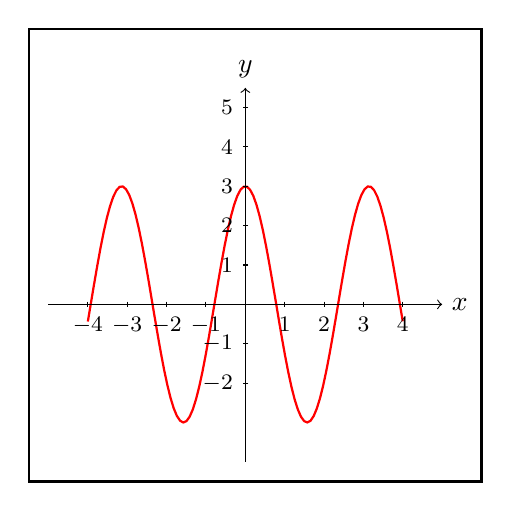
\begin{tikzpicture}[scale=0.5]
				\draw[thick] (-5.5, -4.5) rectangle (6, 7);
				
				% Defina o intervalo x
				
				\def\xmin{-3}
				\def\xmax{3}
				
				% Desenhando a função f_2
				
				\draw[domain=-4:4, thick, samples=100, red] plot (\x, {3*cos(2*\x r)});
				
				% Adicione rótulos aos eixos
				
				\draw[->] (\xmin-2,0) -- (\xmax+2,0) node[right] {$x$};
				\draw[->] (0,\xmin-1) -- (0,\xmax+2.5) node[above] {$y$};				
				
				% Rótulos
				\foreach \i in {-4,-3,-2,-1,1,2,3,4}{
					\draw (\i,2pt)--(\i, -2pt) node[below]{{\footnotesize $\i$}};
				}
				
				\foreach \i in {-2, -1, 1,2,3,4,5}{
					\draw (2pt,\i)--(-2pt, \i) node[left]{{\footnotesize $\i$}};
				}
			\end{tikzpicture}
		
		\end{figure}
	\end{frame}
	\begin{frame}{Percurso do Trabalho}
	\begin{figure}[h]
		\caption{\label{fig:truncamentog_1} Gráfico do truncamento $g_1$ }
		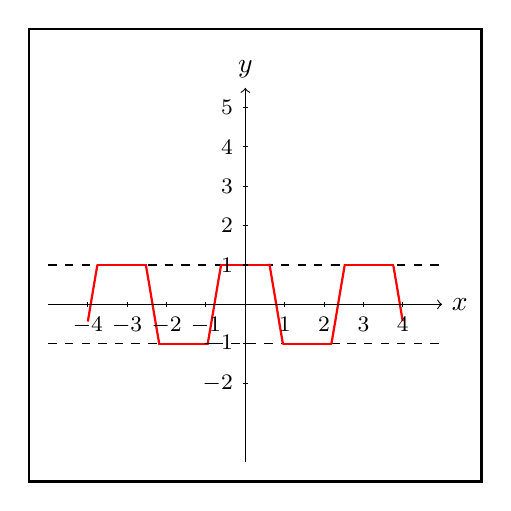
\begin{tikzpicture}[scale=0.5]
			\draw[thick] (-5.5, -4.5) rectangle (6, 7);
			% Defina o intervalo x
			\def\xmin{-3}
			\def\xmax{3}
			
			% Desenhando a função f_2
			\draw[domain=-5:5, dashed, samples=100] plot (\x, {1});
			\draw[domain=-5:5, dashed, samples=100] plot (\x, {-1});
			
			\draw[domain=-4:-3.755, thick, samples=100, red] plot (\x, {3*cos(2*\x r)});
			\draw[domain=-3.76:-2.55, thick, samples=100, red] plot (\x, {1});
			\draw[domain=-2.53:-2.18, thick, samples=100, red] plot (\x, {3*cos(2*\x r)});
			\draw[domain=-2.19:-0.96, thick, samples=100, red] plot (\x, {-1});
			\draw[domain=-0.96:-0.61, thick, samples=100, red] plot (\x, {3*cos(2*\x r)});
			\draw[domain=-0.61:0.635, thick, samples=100, red] plot (\x, {1});
			\draw[domain=0.61:0.96, thick, samples=100, red] plot (\x, {3*cos(2*\x r)});
			\draw[domain=0.96:2.19, thick, samples=100, red] plot (\x, {-1});
			\draw[domain=2.185:2.53, thick, samples=100, red] plot (\x, {3*cos(2*\x r)});
			\draw[domain=2.53:3.76, thick, samples=100, red] plot (\x, {1});]
			\draw[domain=3.76:4, thick, samples=100, red] plot (\x, {3*cos(2*\x r)});
			
			% Adicione rótulos aos eixos
			\draw[->] (\xmin-2,0) -- (\xmax+2,0) node[right] {$x$};
			\draw[->] (0,\xmin-1) -- (0,\xmax+2.5) node[above] {$y$};
			
			% Rótulos
			\foreach \i in {-4,-3,-2,-1,1,2,3,4}{
				\draw (\i,2pt)--(\i, -2pt) node[below]{{\footnotesize $\i$}};
			}
			
			\foreach \i in {-2, -1, 1,2,3,4,5}{
				\draw (2pt,\i)--(-2pt, \i) node[left]{{\footnotesize $\i$}};
			}
		\end{tikzpicture}
	\end{figure}
\end{frame}
\begin{frame}{Percurso do Trabalho}
	\begin{figure}[h]
	\caption{\label{fig:truncamentog_2} Gráfico do truncamento $g_2$ } 
	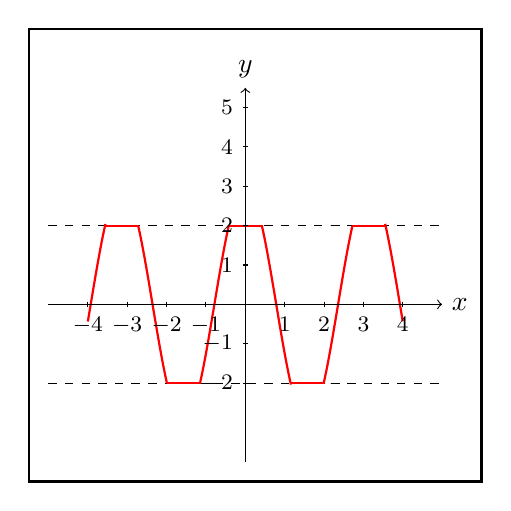
\begin{tikzpicture}[scale=0.5]
		\draw[thick] (-5.5, -4.5) rectangle (6, 7);
		% Defina o intervalo x
		\def\xmin{-3}
		\def\xmax{3}
		
		% Desenhando a função f_2
		\draw[domain=-5:5, dashed, samples=100] plot (\x, {2});
		\draw[domain=-5:5, dashed, samples=100] plot (\x, {-2});
		
		\draw[domain=-4:-3.552, thick, samples=100, red] plot (\x, {3*cos(2*\x r)});
		\draw[domain=-3.55:-2.71, thick, samples=100, red] plot (\x, {2});
		\draw[domain=-2.72:-1.99, thick, samples=100, red] plot (\x, {3*cos(2*\x r)});
		\draw[domain=-2:-1.15, thick, samples=100, red] plot (\x, {-2});
		\draw[domain=-1.15:-0.42, thick, samples=100, red] plot (\x, {3*cos(2*\x r)});
		\draw[domain=-0.43:0.43, thick, samples=100, red] plot (\x, {2});
		\draw[domain=0.42:1.16, thick, samples=100, red] plot (\x, {3*cos(2*\x r)});
		\draw[domain=1.15:2, thick, samples=100, red] plot (\x, {-2});
		\draw[domain=1.99:2.72, thick, samples=100, red] plot (\x, {3*cos(2*\x r)});
		\draw[domain=2.72:3.55, thick, samples=100, red] plot (\x, {2});]
		\draw[domain=3.552:4, thick, samples=100, red] plot (\x, {3*cos(2*\x r)});
		
		% Adicione rótulos aos eixos
		\draw[->] (\xmin-2,0) -- (\xmax+2,0) node[right] {$x$};
		\draw[->] (0,\xmin-1) -- (0,\xmax+2.5) node[above] {$y$};
		
		% Rótulos
		\foreach \i in {-4,-3,-2,-1,1,2,3,4}{
			\draw (\i,2pt)--(\i, -2pt) node[below]{{\footnotesize $\i$}};
		}
		
		\foreach \i in {-2, -1, 1,2,3,4,5}{
			\draw (2pt,\i)--(-2pt, \i) node[left]{{\footnotesize $\i$}};
		}
	\end{tikzpicture}
\end{figure}
\end{frame}
	\begin{frame}{Percurso do Trabalho}{Espaços de Medida}
		\begin{block}<+->{Definição}
			\justify Uma medida é uma função $\mu: (X, \mathcal{C}) \to \xreta$ tal que satisfaz as seguintes condições:
			\begin{itemize}[<+->]
				\item $\mu(\varnothing) = 0$;
				\item $\mu(A) \geq 0, \ \forall \ A \in \mathcal{C}$;
				\item Se $(A_n)$ é uma sequência disjunta de elementos de  $\mathcal{C}$, então 
				$\displaystyle\mu\left(\bigcup_{n = 1}^\infty A_n\right) = \sum_{n = 1}^\infty\mu(A_n)$
			\end{itemize}
		\end{block}
	\end{frame}

	\begin{frame}{Percurso do Trabalho}
		\begin{block}{Teorema}
			\justify Seja $\mu$ uma medida definida sobre uma \sigal $\mathcal{C}$.
			Se $A$ e $B$ são elementos de $\mathcal{C}$ e $A \subset B$, então $\mu(A) \leq \mu(B)$.
			Se $\mu(A) < +\infty$, então $\mu(B-A) = \mu(B) - \mu(A)$.
		\end{block}
	\end{frame}

	\begin{frame}{Percurso do Trabalho}
		\begin{block}{Exemplos}
			Sejam $X$ um conjunto e $\mathcal{C}$ a \sigal formada por todos os subconjunto de $X$.    
			Defina $\mu_1, \mu_2:\mathcal{C} \to \xreta$ pondo $\mu_1(A) = 0$ para qualquer  $A \in \mathcal{C}$ e 
			$\mu_2$ é  pondo 
			$$\mu_2(A) = \left\{\begin{array}{cc}
				0, & \textrm{\ se \ } A = \varnothing \\
				+\infty,& \textrm{\ se \ } A \neq \varnothing
			\end{array}\right.$$
			Sendo definidas dessa forma, as funções $\mu_1$ e $\mu_2$ são medidas.
		\end{block}
	\end{frame}

	\begin{frame}{Percurso do Trabalho}
		\begin{block}{Exemplo}
			\justify Seja $(\Omega, \cc)$ um espaço mensurável.
			A função $\mathcal{P}:\cc \to [0,1]$ é dita uma probabilidade se satisfaz as propriedades:
			\begin{enumerate}[<+->]
				\item $\mathcal{P}(\Omega) = 1$;
				\item $\mathcal{P}(A) \geq 0,\ \forall\  A \in \cc$;
				\item Se $(A_n)$ é uma sequência disjunta de elementos de  $\mathcal{C}$, então 
				$\displaystyle\mathcal{P}\left(\bigcup_{n = 1}^\infty A_n\right) = \sum_{n = 1}^\infty\mathcal{P}(A_n)$.
			\end{enumerate}
		\end{block}
	\end{frame}
	\begin{frame}{Percurso do Trabalho}
		\begin{block}<+->{Teorema}
			\justify Seja $\mu$ uma medida definida sobre uma \sigal $\mathcal{C}$.
			Se $A$ e $B$ são elementos de $\mathcal{C}$ e $A \subset B$, então $\mu(A) \leq \mu(B)$.
			Se $\mu(A) < +\infty$, então $\mu(B-A) = \mu(B) - \mu(A)$
		\end{block}
	\end{frame}

	\begin{frame}{Percurso do Trabalho}
		\begin{block}<+->{Proposição}
			\justify Seja $\mu$ uma medida definida sobre uma \sigal $\mathcal{C}$.
			Se $(B_n)$ é uma sequência não-crescente de $\mathcal{C}$ e $\mu(B_1) < +\infty$, então 
			$\mu\left(\displaystyle \bigcap_{n = 1}^\infty B_n\right) = \displaystyle\lim_{n \to \infty} \mu(B_n)$.
		\end{block}
	\end{frame}
	
	\begin{frame}{Percurso do Trabalho}
		\begin{block}<+->{Teorema}
			\justify Sendo $(\R, \borel)$ um espaço mensurável, existe uma única medida $\lambda$ definida sobre $\borel$ que coincide com o comprimento dos intervalos abertos.
		\end{block}
		\begin{block}<+->{Definição}
			\justify Seja $(X, \cc, \mu)$ um espaço de medida.
			Dizemos que um conjunto $E \in \cc$ tem medida nula em relação à medida $\mu$ se $\mu(E) = 0$.
		\end{block}
	\end{frame}

% Integração]
	\subsection{Teoria da Integração}
	\begin{frame}{Percurso do Trabalho}{A integração de Funções Simples}
		\begin{block}<+->{Definição}
			\justify Uma função real é dita \textbf{simples} quando possui apenas uma quantidade finita de valores.
		\end{block}
	\end{frame}
	\begin{frame}
		\begin{block}<+->{Definição}
			\justify Forma Padrão
			$$
			\varphi =  \sum_{j = 1}^n a_j\chi_{E_j}
			$$
			onde $a_j \in \R$ e $\chi_{E_j}$ é a função característica do conjunto $E_j \in \cc$.
			Nessa representação estamos supondo que cada $a_j \neq a_i$ quando $j \neq i$ e que
			$\displaystyle \bigcup_{j = 1}^n E_j = X$, onde a sequência finita de conjuntos $(E_n)$ formam uma partição do conjunto $X$.
		\end{block}
	\end{frame}
	\begin{frame}{Percurso do Trabalho}
		\begin{block}{Exemplo}
			$g: [0,4] \to \R$ pondo 
			$$g(x) = \left\{
			\begin{array}{cc}
				1, & \textrm{\ se } x \in [0,1) \\
				3, & \textrm{\ se } x \in [1,2) \\
				4, & \textrm{\ se } x \in [2,3) \\
				2, & \textrm{\ se } x \in [3,4]
			\end{array}\right.
			$$
		\end{block}
	\end{frame}
	\begin{frame}{Percurso do Trabalho}
		\begin{figure}
			\caption{\label{fig:integral-função-simples-g-sobre-[0,4]} Gráfico da função $\displaystyle g =\sum_{j = 1}^4 a_j\chi_{E_j}$}	
			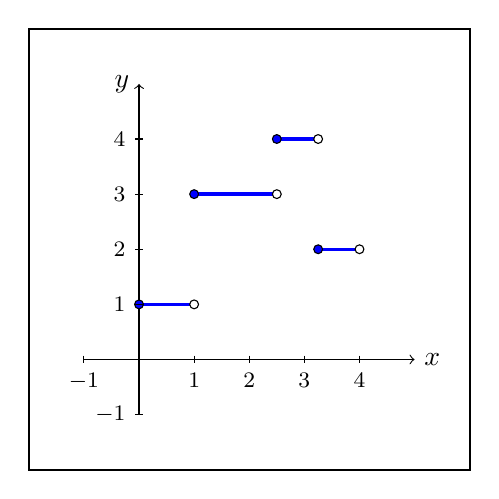
\begin{tikzpicture}[scale=0.7]
				
				\draw[thick] (-2,-2) rectangle (6, 6);
				% Eixos
				\draw[->] (-1,0) -- (5,0) node[right] {$x$};
				\draw[->] (0,-1) -- (0, 5) node[left] {$y$};
				
				% Plot do gráfico
				\draw[domain=0:1,very thick,variable=\x,blue] plot ({\x},{1});
				\draw[domain=1:2.5,very thick,variable=\x,blue] plot ({\x},{3});
				\draw[domain=2.5:3.25,very thick,variable=\x,blue] plot ({\x},{4});
				\draw[domain=3.25:4,very thick,variable=\x,blue] plot ({\x},{2});
				
				% Bolinhas dos Intervalos
				\draw[fill=blue] (0,1) circle (0.08);
				\draw[fill=blue] (1,3) circle (0.08);
				\draw[fill=blue] (2.5,4) circle (0.08);
				\draw[fill=blue] (3.25,2) circle (0.08);
				
				\draw[fill=white] (1,1) circle (0.08);
				\draw[fill=white] (2.5,3) circle (0.08);
				\draw[fill=white] (3.25,4) circle (0.08);
				\draw[fill=white] (4,2) circle (0.08);
				
				
				% Rótulos
				\foreach \i in {-1,1,2,3,4}{
					\draw (\i,2pt)--(\i, -2pt) node[below]{{\footnotesize $\i$}};
				}
				
				\foreach \i in {-1,1,2,3,4}{
					\draw (2pt,\i)--(-2pt, \i) node[left]{{\footnotesize $\i$}};
				}
				
				% Linhas trastejadas
				% \foreach \i in {1,2,3,4}{
					% \draw[dashed, help lines] (\i,0) -- (\i,\i);
					% }
				% \foreach \i in {1,2,3}{
					% \draw[dashed, help lines] (\i,\i) -- (\i,\i+1);
					% }  
			\end{tikzpicture}
		\end{figure}
	\end{frame}

	\begin{frame}{Percurso do Trabalho}
		\begin{figure}
			\caption{ Área delimitada pelo gráfico da função $g =\displaystyle \sum_{j = 1}^4 a_j\chi_{E_j}$}	
				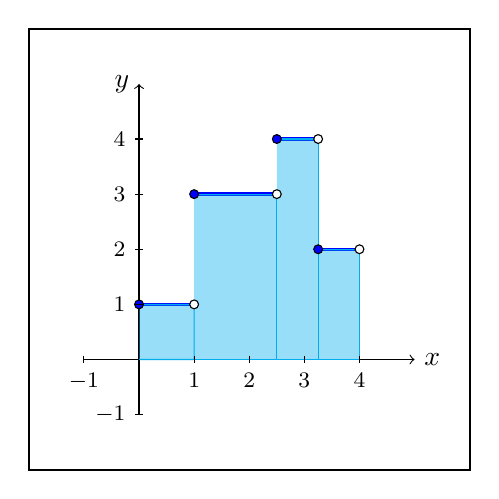
\begin{tikzpicture}[scale=0.7]
					
					\draw[thick] (-2,-2) rectangle (6, 6);
					% Eixos
					\draw[->] (-1,0) -- (5,0) node[right] {$x$};
					\draw[->] (0,-1) -- (0, 5) node[left] {$y$};
					
					% Plot do gráfico	
					\draw[domain=0:1,very thick,variable=\x,blue] plot ({\x},{1});
					\draw[domain=1:2.5,very thick,variable=\x,blue] plot ({\x},{3});
					\draw[domain=2.5:3.25,very thick,variable=\x,blue] plot ({\x},{4});
					\draw[domain=3.25:4,very thick,variable=\x,blue] plot ({\x},{2});
					
					
					\filldraw [domain=0:1,smooth,variable=\x, cyan, fill opacity=0.4]  plot ({\x},{1})--(1,0)--(0,0);
					\filldraw [domain=1:2.5,smooth,variable=\x, cyan, fill opacity=0.4]  plot ({\x},{3})--(2.5,0)--(1,0);
					\filldraw [domain=2.5:3.25,smooth,variable=\x, cyan, fill opacity=0.4]  plot ({\x},{4})--(3.25,0)--(2.5,0);
					\filldraw [domain=3.25:4,smooth,variable=\x, cyan, fill opacity=0.4]  plot ({\x},{2})--(4,0)--(3.25,0);
					
					% Bolinhas dos Intervalos
					\draw[fill=blue] (0,1) circle (0.08);
					\draw[fill=blue] (1,3) circle (0.08);
					\draw[fill=blue] (2.5,4) circle (0.08);
					\draw[fill=blue] (3.25,2) circle (0.08);
					
					\draw[fill=white] (1,1) circle (0.08);
					\draw[fill=white] (2.5,3) circle (0.08);
					\draw[fill=white] (3.25,4) circle (0.08);
					\draw[fill=white] (4,2) circle (0.08);
					
					
					% Rótulos
					\foreach \i in {-1,1,2,3,4}{
						\draw (\i,2pt)--(\i, -2pt) node[below]{{\footnotesize $\i$}};
					}
					
					\foreach \i in {-1,1,2,3,4}{
						\draw (2pt,\i)--(-2pt, \i) node[left]{{\footnotesize $\i$}};
					}
			\end{tikzpicture}
		\end{figure}
	\end{frame}
	% Definição de Integral para Funções Simples

	\begin{frame}{Percurso do Trabalho}
		\begin{block}{Definição}
			\justify Se $\varphi$ é uma função simples de $M^+(X, \cc)$ com a representação 
			$\displaystyle\varphi = \displaystyle  \sum_{j = 1}^n a_j\chi_{E_j},$ então a integral da função $\varphi$ com respeito à medida $\mu$ é o valor real estendido
			$$
			\displaystyle\int\varphi d\mu = \sum_{j = 1}^n a_j\mu(E_j)
			$$
		\end{block}
	\end{frame}

	\begin{frame}{Percurso do Trabalho}
		\begin{block}{Teorema}
			\justify Se $\varphi$ e $\psi$ são funções simples do espaço $M^+(X,\cc)$ e $c\geq0$ é uma constante real, então
			\begin{itemize}
				\item $ \displaystyle \int c\varphi d\mu = c \int \varphi d\mu$;
				\item $ \displaystyle \int (\varphi + \psi) d\mu = \int \varphi d\mu + \int \psi d\mu$.
			\end{itemize}
		\end{block}
	\end{frame}
	
	\begin{frame}{Percurso do Trabalho}
	\begin{block}{Teorema}
		\justify Se $\phi$ é uma função simples com  a representação padrão dada por $\phi = \displaystyle \sum_{j = 1}^n a_j\chi_{E_j}$, então a função $\lambda: \cc \to \xreta$ definida por
		$$
		\displaystyle\lambda(E) = \int \varphi\chi_E\ d\mu
		$$
		para todo $E \in \cc$ é uma medida sobre $\cc$
		\end{block}
	\end{frame}

% Integrais de Funções Quaisquer Não negativas

% Diferença entre as Integrais	
	\begin{frame}{Percurso do Trabalho}{Integral de Funções Não Negativas}
		\begin{figure}
			\caption{\label{fig:gráfico da função sen x + 3} Gráfico da função $f(x) = \textrm{sen}(x) + 3$} 	
			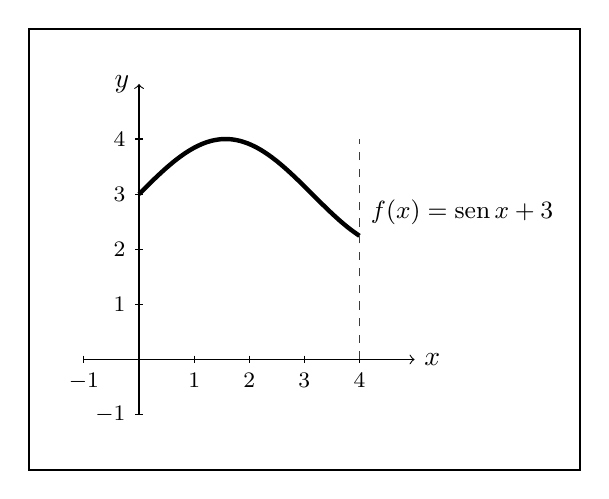
\begin{tikzpicture}[scale=0.7]
				\draw[thick] (-2,-2) rectangle (8, 6);
				% Eixos
				\draw[->] (-1,0) -- (5,0) node[right] {$x$};
				\draw[->] (0,-1) -- (0, 5) node[left] {$y$};

				% Rótulos
				\foreach \i in {-1,1,2,3,4}{
					\draw (\i,2pt)--(\i, -2pt) node[below]{{\footnotesize $\i$}};
				}
				
				\foreach \i in {-1,1,2,3,4}{
					\draw (2pt,\i)--(-2pt, \i) node[left]{{\footnotesize $\i$}};
				}

				\draw[domain=0:4,smooth,variable=\x, ultra thick]  plot ({\x},{3+sin(\x r)})  node[above right] {{\small $f(x) = \textrm{sen}\,x + 3$}};
				\draw[dashed, green!40!black]  (4,0)--(4,4);
			\end{tikzpicture}
		\end{figure}
	\end{frame}

	\begin{frame}{Percurso do Trabalho}
		\begin{figure}
		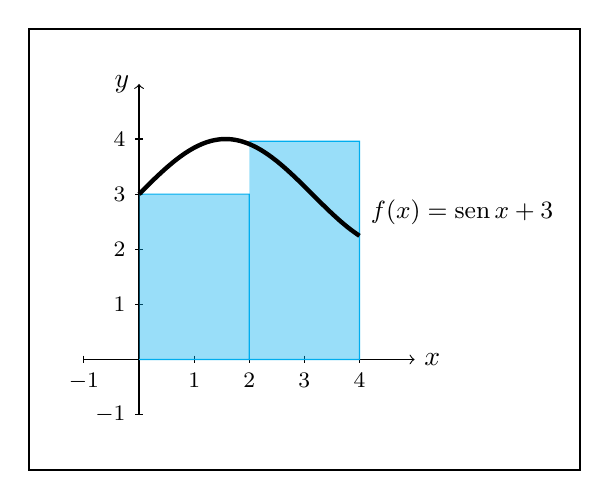
\begin{tikzpicture}[scale=0.7]
			\draw[thick] (-2,-2) rectangle (8, 6);
			% Eixos
			\draw[->] (-1,0) -- (5,0) node[right] {$x$};
			\draw[->] (0,-1) -- (0, 5) node[left] {$y$};
			
			% Rótulos
			\foreach \i in {-1,1,2,3,4}{
				\draw (\i,2pt)--(\i, -2pt) node[below]{{\footnotesize $\i$}};
			}
			
			\foreach \i in {-1,1,2,3,4}{
				\draw (2pt,\i)--(-2pt, \i) node[left]{{\footnotesize $\i$}};
			}
			% Plot do gráfico
			\filldraw[domain=0:2,smooth,variable=\x, cyan, fill opacity=0.4] plot ({\x},{3})--(2,0)--(0,0);
			\filldraw[domain=2:4,smooth,variable=\x, cyan, fill opacity=0.4] plot ({\x},{3.96})--(4,0)--(2,0);	
			
			\draw[domain=0:4,smooth,variable=\x, ultra thick]  plot ({\x},{3+sin(\x r)})  node[above right] {{\small $f(x) = \textrm{sen}\,x + 3$}};
			
		\end{tikzpicture}
		\end{figure}
	\end{frame}

	\begin{frame}{Percurso do Trabalho}
	\begin{figure}
		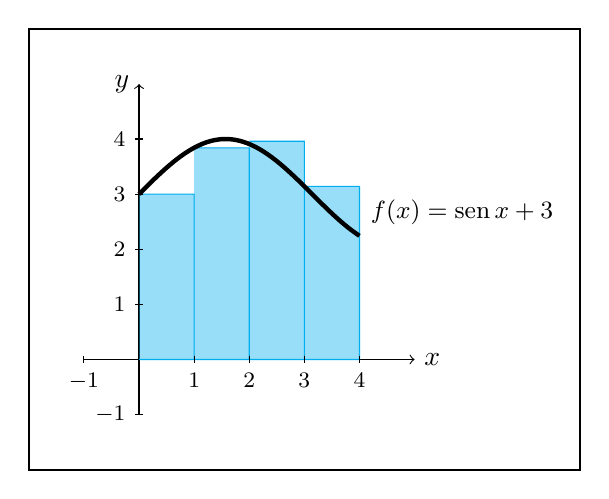
\begin{tikzpicture}[scale=0.7]
			\draw[thick] (-2,-2) rectangle (8, 6);
			% Eixos
			\draw[->] (-1,0) -- (5,0) node[right] {$x$};
			\draw[->] (0,-1) -- (0, 5) node[left] {$y$};
			
			% Plot do gráfico
			\filldraw [domain=0:1,smooth,variable=\x, cyan, fill opacity=0.4]  plot ({\x},{3})--(1,0)--(0,0);
			\filldraw[domain=1:2,smooth,variable=\x, cyan, fill opacity=0.4] plot ({\x},{3.84})--(2,0)--(1,0);	
			\filldraw[domain=2:3,smooth,variable=\x, cyan, fill opacity=0.4] plot ({\x},{3.96})--(3,0)--(2,0);
			\filldraw[domain=3:4,smooth,variable=\x, cyan, fill opacity=0.4] plot ({\x},{3.14})--(4,0)--(3,0);
			
			% Rótulos
			\foreach \i in {-1,1,2,3,4}{
				\draw (\i,2pt)--(\i, -2pt) node[below]{{\footnotesize $\i$}};
			}
			
			\foreach \i in {-1,1,2,3,4}{
				\draw (2pt,\i)--(-2pt, \i) node[left]{{\footnotesize $\i$}};
			}
			
			\draw[domain=0:4,smooth,variable=\x, ultra thick]  plot ({\x},{3+sin(\x r)})  node[above right] {{\small $f(x) = \textrm{sen}\,x + 3$}};
			
		\end{tikzpicture}
	\end{figure}
\end{frame}
	
\begin{frame}{Percurso do Trabalho}
	\begin{figure}
		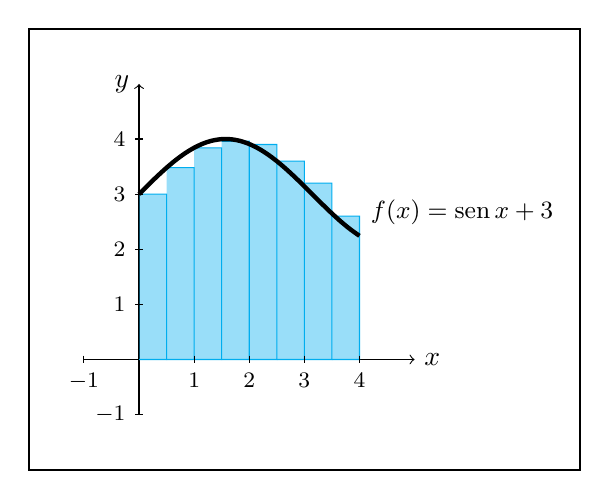
\begin{tikzpicture}[scale=0.7]
			\draw[thick] (-2,-2) rectangle (8, 6);
			% Eixos
			\draw[->] (-1,0) -- (5,0) node[right] {$x$};
			\draw[->] (0,-1) -- (0, 5) node[left] {$y$};
			
			% Plot do gráfico
			\filldraw [domain=0:0.5,smooth,variable=\x, cyan, fill opacity=0.4]  plot ({\x},{3})--(0.5,0)--(0,0);
			
			\filldraw [domain=0.5:1,smooth,variable=\x, cyan, fill opacity=0.4]  plot ({\x},{3.48})--(1,0)--(0.5,0);
			
			\filldraw[domain=1:1.5,smooth,variable=\x, cyan, fill opacity=0.4] plot ({\x},{3.84})--(1.5,0)--(1,0);	
			
			\filldraw[domain=1.5:2,smooth,variable=\x, cyan, fill opacity=0.4] plot ({\x},{3.96})--(2,0)--(1.5,0);
			
			\filldraw[domain=2:2.5,smooth,variable=\x, cyan, fill opacity=0.4] plot ({\x},{3.9})--(2.5,0)--(2,0);
			
			\filldraw[domain=2.5:3,smooth,variable=\x, cyan, fill opacity=0.4] plot ({\x},{3.6})--(3,0)--(2.5,0);
			
			\filldraw[domain=3:3.5,smooth,variable=\x, cyan, fill opacity=0.4] plot ({\x},{3.2})--(3.5,0)--(3,0);
			
			\filldraw[domain=3.5:4,smooth,variable=\x, cyan, fill opacity=0.4] plot ({\x},{2.6})--(4,0)--(3.5,0);
			
			% Rótulos
			\foreach \i in {-1,1,2,3,4}{
				\draw (\i,2pt)--(\i, -2pt) node[below]{{\footnotesize $\i$}};
			}
			
			\foreach \i in {-1,1,2,3,4}{
				\draw (2pt,\i)--(-2pt, \i) node[left]{{\footnotesize $\i$}};
			}
			
			\draw[domain=0:4,smooth,variable=\x, ultra thick]  plot ({\x},{3+sin(\x r)})  node[above right] {{\small $f(x) = \textrm{sen}\,x + 3$}};
			
		\end{tikzpicture}
	\end{figure}
\end{frame}

\begin{frame}{Percurso do Trabalho}
	\begin{figure}
		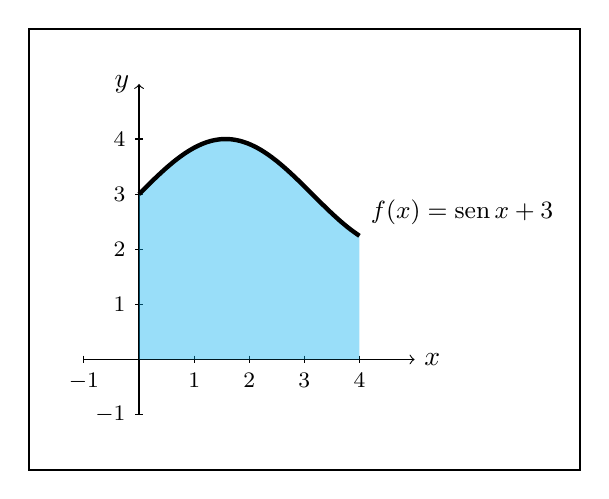
\begin{tikzpicture}[scale=0.7]
			\draw[thick] (-2,-2) rectangle (8, 6);
			% Eixos
			\draw[->] (-1,0) -- (5,0) node[right] {$x$};
			\draw[->] (0,-1) -- (0, 5) node[left] {$y$};
			% Rótulos
			\foreach \i in {-1,1,2,3,4}{
				\draw (\i,2pt)--(\i, -2pt) node[below]{{\footnotesize $\i$}};
			}
			
			\foreach \i in {-1,1,2,3,4}{
				\draw (2pt,\i)--(-2pt, \i) node[left]{{\footnotesize $\i$}};
			}
			\fill[domain=0:4,smooth,variable=\x, cyan, fill opacity=0.4]  plot ({\x},{3+sin(\x r)})--(4,0)--(0,0);
			% Yes, this is drawn twice, but I wanted the shading to match the over/under pictures following.
			
			
			\draw[domain=0:4,smooth,variable=\x, ultra thick]  plot ({\x},{3+sin(\x r)})  node[above right] {{\small $f(x) = \textrm{sen}\,x + 3$}};
		\end{tikzpicture}
		\end{figure}
	\end{frame}

% Repartição da Imagem.
	\begin{frame}{Percurso do Trabalho}
		\begin{block}{Partição pela imagem}
			Dada a função  $f(x) = x^2$, construiremos a função simples $\phi_1$ pondo:
			$$
			\phi_1(x) =\left\{
			\begin{array}{ll}
				0, & \textrm{se\ } 0 \leq f(x) < 2^{-1} \\
				2^{-1}, & \textrm{se\ } 2^{-1} \leq f(x) < 2\cdot2^{-1} \\
				1, & \textrm{se\ } f(x) \geq 1
			\end{array}
			\right.
			$$
		\end{block}
	\end{frame}

	\begin{frame}{Percurso do Trabalho}
		\begin{figure}
			\caption{\label{fig: Lebesgue gráfico da função phi 1}Gráfico da função $\phi_1$} 
				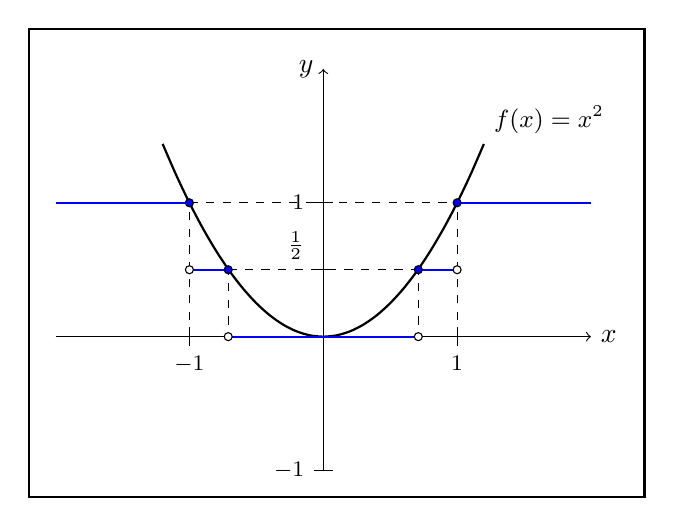
\begin{tikzpicture}[scale=1.7]
					\draw[thick] (-2.2,-1.2) rectangle (2.4, 2.3);
					% Eixos
					\draw[->] (-2,0) -- (2,0) node[right] {$x$};
					\draw[->] (0,-1) -- (0, 2) node[left] {$y$};
					% Rótulos
					\foreach \i in {-1,1}{
						\draw (\i,2pt)--(\i, -2pt) node[below]{{\footnotesize $\i$}};
					}
					
					\foreach \i in {-1, 1}{
						\draw (2pt,\i)--(-2pt, \i) node[left]{{\footnotesize $\i$}};
					}
					
					\draw (2pt,0.5)--(-2pt, 0.5) node[above left]{\footnotesize $\frac{1}{2}$};
					
					%\fill[domain=-1:1,smooth,variable=\x, cyan, fill opacity=0.4]  plot ({\x},{\x*\x})--(4,0)--(0,0);
					% Yes, this is drawn twice, but I wanted the shading to match the over/under pictures following.
					
					\draw[domain=-1.2:1.2,smooth,variable=\x, thick]  plot ({\x},{\x*\x})  node[above right] {{\small $f(x) = x^2$}};
					
					% Função $\phi_1$
					\draw[domain=-0.71:0.71,smooth,variable=\x,thick, blue]  plot ({\x},{0});
					
					\draw[domain=-1:-0.71,smooth,variable=\x,thick, blue]  plot ({\x},{0.5});
					\draw[domain=0.71:1,smooth,variable=\x,thick, blue]  plot ({\x},{0.5});
					
					\draw[domain=-2:-1,smooth,variable=\x,thick, blue]  plot ({\x},{1});
					\draw[domain=1:2,smooth,variable=\x,thick, blue]  plot ({\x},{1});
					
					% Retas auxiliares
					\draw[dashed] (-0.71,0.09) -- (-0.71,0.5);
					\draw[dashed] (0.71,0.09) -- (0.71,0.5);
					
					\draw[dashed] (-0.71,0.5) -- (0.71,0.5);
					
					\draw[dashed] (-1,1) -- (1,1);
					
					\draw[dashed] (-1,0) -- (-1,1);
					\draw[dashed] (1,0) -- (1,1);
					
					% Bolinhas
					\draw[fill=white] (-0.71,0) circle (0.03);
					\draw[fill=white] (0.71,0) circle (0.03);
					
					\draw[fill=blue] (-0.71,0.5) circle (0.03);
					\draw[fill=blue] (0.71,0.5) circle (0.03);
					
					\draw[fill=white] (-1,0.5) circle (0.03);
					\draw[fill=white] (1,0.5) circle (0.03);
					
					\draw[fill=blue] (-1,1) circle (0.03);
					\draw[fill=blue] (1,1) circle (0.03);
				\end{tikzpicture}
		\end{figure}
	\end{frame}

	\begin{frame}{Percurso do Trabalho}
		\begin{block}{A	proximação a função $f$ agora pela função simples $\phi_2$}
			$$
			\phi_2(x) =\left\{
			\begin{array}{ll}
				0, & \textrm{se\ } 0 \leq f(x) < 2^{-2} \\
				2^{-2}, & \textrm{se\ } 2^{-2} \leq f(x) < 2\cdot2^{-2} \\
				2\cdot 2^{-2}, & \textrm{se\ } 2\cdot 2^{-2} \leq f(x) < 3\cdot2^{-2}\\
				3\cdot 2^{-2}, & \textrm{se\ } 3\cdot 2^{-2} \leq f(x) < 4\cdot2^{-2}\\
				4\cdot 2^{-2}, & \textrm{se\ } 4\cdot 2^{-2} \leq f(x) < 5\cdot2^{-2}\\
				5\cdot 2^{-2}, & \textrm{se\ } 5\cdot 2^{-2} \leq f(x) < 6\cdot2^{-2}\\
				6\cdot 2^{-2}, & \textrm{se\ } 6\cdot 2^{-2} \leq f(x) < 7\cdot2^{-2}\\
				7\cdot 2^{-2}, & \textrm{se\ } 7\cdot 2^{-2} \leq f(x) < 8\cdot2^{-2}\\
				2, & \textrm{se\ } f(x) \geq 2\\
			\end{array}
			\right.
			$$
		\end{block}
	\end{frame}
	\begin{frame}{Percurso do Trabalho}
		\begin{figure}
			\caption{Gráfico da função $\phi_2$} 
			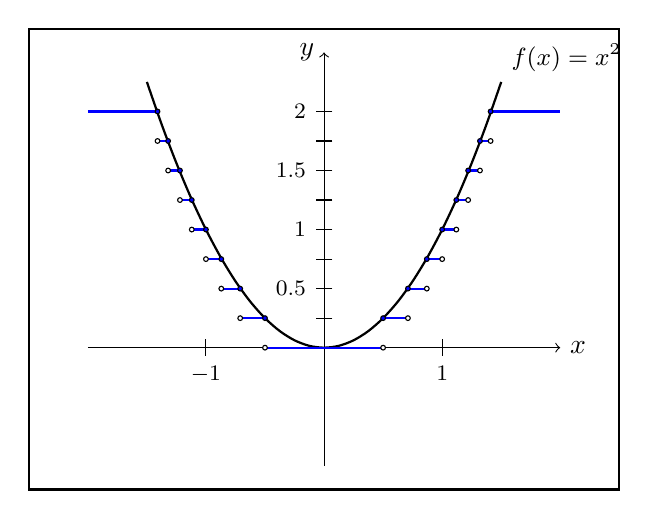
\begin{tikzpicture}[scale=1.5]
				\draw[thick] (-2.5,-1.2) rectangle (2.5, 2.7);
				% Eixos
				\draw[->] (-2,0) -- (2,0) node[right] {$x$};
				\draw[->] (0,-1) -- (0, 2.5) node[left] {$y$};
				
				% Rótulos
				\foreach \i in {-1,1}{
					\draw (\i,2pt)--(\i, -2pt) node[below]{{\footnotesize $\i$}};
				}
				
				\foreach \i in {0.5, 1, 1.5, 2}{
					\draw (2pt,\i)--(-2pt, \i) node[left]{{\footnotesize $\i$}};
				}
				
				\foreach \i in {0.25, 0.75, 1.25, 1.75}{
					\draw (2pt,\i)--(-2pt, \i);
				}
				
				\draw[domain=-1.5:1.5,smooth,variable=\x, thick]  plot ({\x},{\x*\x})  node[above right] {{\small $f(x) = x^2$}};
								
				% Função $\phi_2$
				\draw[domain=-0.5:0.5,smooth,variable=\x,thick, blue]  plot ({\x},{0});
				
				\draw[domain=-0.71:-0.5,smooth,variable=\x,thick, blue]  plot ({\x},{0.25});
				\draw[domain=0.5:0.71,smooth,variable=\x,thick, blue]  plot ({\x},{0.25});
				
				\draw[domain=-0.87:-0.71,smooth,variable=\x,thick, blue]  plot ({\x},{0.5});
				\draw[domain=0.71:0.87,smooth,variable=\x,thick, blue]  plot ({\x},{0.5});
				
				\draw[domain=-1:-0.87,smooth,variable=\x,thick, blue]  plot ({\x},{0.75});
				\draw[domain=0.87:1,smooth,variable=\x,thick, blue]  plot ({\x},{0.75});
				
				\draw[domain=-1.12:-1,smooth,variable=\x,thick, blue]  plot ({\x},{1});
				\draw[domain=1:1.12,smooth,variable=\x,thick, blue]  plot ({\x},{1});
				
				\draw[domain=-1.22:-1.12,smooth,variable=\x,thick, blue]  plot ({\x},{1.25});
				\draw[domain=1.12:1.22,smooth,variable=\x,thick, blue]  plot ({\x},{1.25});
				
				\draw[domain=-1.32:-1.22,smooth,variable=\x,thick, blue]  plot ({\x},{1.5});
				\draw[domain=1.22:1.32,smooth,variable=\x,thick, blue]  plot ({\x},{1.5});
				
				\draw[domain=-1.41:-1.32,thick,variable=\x,thick, blue]  plot ({\x},{1.75});
				\draw[domain=1.32:1.41,thick,variable=\x,thick, blue]  plot ({\x},{1.75});
				
				\draw[domain=-2:-1.41,thick,variable=\x,thick, blue]  plot ({\x},{2});
				\draw[domain=1.41:2,thick,variable=\x,thick, blue]  plot ({\x},{2});
				
				% Bolinhas
				\draw[fill=white] (-0.5,0) circle (0.02);
				\draw[fill=white] (0.5,0) circle (0.02);
				
				\draw[fill=blue] (-0.5, 0.25) circle (0.02);
				\draw[fill=blue] (0.5, 0.25) circle (0.02);
				
				\draw[fill=white] (-0.71,0.25) circle (0.02);
				\draw[fill=white] (0.71,0.25) circle (0.02);
				
				\draw[fill=blue] (-0.71,0.5) circle (0.02);
				\draw[fill=blue] (0.71,0.5) circle (0.02);
				
				\draw[fill=white] (-0.87,0.5) circle (0.02);
				\draw[fill=white] (0.87,0.5) circle (0.02);
				
				\draw[fill=blue] (-0.87,0.75) circle (0.02);
				\draw[fill=blue] (0.87,0.75) circle (0.02);
				
				\draw[fill=white] (-1,0.75) circle (0.02);
				\draw[fill=white] (1,0.75) circle (0.02);
				
				\draw[fill=blue] (-1,1) circle (0.02);
				\draw[fill=blue] (1,1) circle (0.02);
				
				\draw[fill=white] (-1.12,1) circle (0.02);
				\draw[fill=white] (1.12,1) circle (0.02);
				
				\draw[fill=blue] (-1.12,1.25) circle (0.02);
				\draw[fill=blue] (1.12,1.25) circle (0.02);
				
				\draw[fill=white] (-1.22,1.25) circle (0.02);
				\draw[fill=white] (1.22, 1.25) circle (0.02);
				
				\draw[fill=blue] (-1.22,1.5) circle (0.02);
				\draw[fill=blue] (1.22, 1.5) circle (0.02);
				
				\draw[fill=white] (-1.32,1.5) circle (0.02);
				\draw[fill=white] (1.32, 1.5) circle (0.02);
				
				\draw[fill=blue] (-1.32,1.75) circle (0.02);
				\draw[fill=blue] (1.32, 1.75) circle (0.02);
				
				\draw[fill=white] (-1.41,1.75) circle (0.02);
				\draw[fill=white] (1.41, 1.75) circle (0.02);
				
				\draw[fill=blue] (-1.41,2) circle (0.02);
				\draw[fill=blue] (1.41, 2) circle (0.02);
			\end{tikzpicture}		
		\end{figure}
	\end{frame}
	
	\begin{frame}{Percurso do Trabalho}
		\begin{block}{Partição da Imagem em $n$ partes}
			$$
			\varphi_n(x) =\left\{
			\begin{array}{ll}
				0, & \textrm{se\ } 0 \leq f(x) < 2^{-n} \\
				2^{-n}, & \textrm{se\ } 2^{-n} \leq f(x) < 2\cdot2^{-n} \\
				2\cdot2^{-n}, & \textrm{se\ } 2\cdot2^{-n} \leq f(x) < 3\cdot2^{-n} \\
				\vdots & \vdots \\
				k\cdot2^{-n}, & \textrm{se\ } k\cdot2^{-n} \leq f(x) < (k+1)\cdot2^{-n} \\
				\vdots & \vdots \\
				n, & \textrm{se\ } f(x) \geq n
			\end{array}
			\right.
			$$
		\end{block}
	\end{frame}
	\begin{frame}{Percurso do Trabalho`}
		\begin{block}{Teorema}
			Se $f$ é uma função não negativa em $\menfus$, então existe uma sequência de funções $(\varphi_n)$ tal que $\phi \in \menfus, \forall \ n \in \N$ de forma que
			\begin{enumerate}
				\item Cada $\varphi_n$ é uma função simples, isto é, possui apenas uma quantidade finita de valores reais;
				\item $0 \leq \varphi_n(x) \leq f(x)$ para todo $x \in X$ e $n \in \N$;
				\item $\displaystyle\lim_{n \to \infty} \varphi_n(x) = f(x)$ para todo $x \in X$.
			\end{enumerate}
		\end{block}
	\end{frame}
	
	\begin{frame}{Percurso do Trabalho}
		\begin{block}{Definição}
			\justify Se $f \in M^+(X,\cc)$, nós definimos a integral de $f$ com respeito à medida $\mu$, sendo o valor real estendido
			$$
			\int f d\mu = sup \int \varphi d\mu
			$$
			Onde o supremo é sobre todas as funções simples $\varphi \in \menfus$ tal que  $0 \leq \varphi \leq f(x)$ para todo $x \in X$
		\end{block}
	\end{frame}
	
	\begin{frame}{Percurso do Trabalho}
		\begin{block}{Teorema da Convergência Monótona}
			\justify Se $(f_n)$ é uma sequência monótona crescente de funções mensuráveis, não negativas, que converge para uma função $f$, então
			$$ \displaystyle
			\int f d\mu = \lim_{n \to \infty} \int f_n d\mu
			$$
		\end{block}
	\end{frame}
	\begin{frame}{Percurso do Trabalho}
		\begin{block}<+->{Corolário}
			\justify Se $f \in M^+(X, \cc)$ e $c \geq 0$, então $cf \in M^+(X, \cc)$ e vale
			$ \displaystyle
			\int cf d\mu = c\int f d\mu.
			$	
		\end{block}
		\begin{block}{Corolário}
			\justify Se $f$ e $g$ são funções não negativas e $\cc$-mensuráveis, então  a soma $f + g$ também é uma função $\cc$-mensurável e vale
			$ \displaystyle
			\int (f + g) d\mu = \int f d\mu + \int g d\mu
			$
		\end{block}
	\end{frame}
	
	\begin{frame}{Percurso do Trabalho}
		\begin{block}{Lema de Fatou}
			\justify Se $(f_n)$ é uma sequência tal que $f_n \in M^+(X, \cc)$ para qualquer que seja $n \in \N$, então 
			$$\displaystyle
			\int(\lim \inf f_n)d\mu \leq \lim \inf \int f_n d\mu$$
		\end{block}
	\end{frame}
	
	\begin{frame}{Percurso do Trabalho}
		\begin{block}{Definição}
				\justify Diremos que alguma propriedade ocorre em quase todo ponto de um conjunto $X$ com respeito à medida $\mu$, se ela não é valida somente em um subconjunto $E$ de $X$ que tem medida nula.
			Denotaremos esse acontecimento por $\mu$-q.t.p.
		\end{block}
	\end{frame}

	\begin{frame}{Percurso do Trabalho}
		\begin{block}{Corolário}
			\justify Se $(g_n)$ é uma sequência de funções em $M^+(X, \cc)$, então 
			$$
			\int \left(\sum_{n = 1} ^\infty g_n\right)d\mu
			=
			\sum_{n = 1} ^\infty \left(\int g_n d\mu\right).
			$$
		\end{block}
	\end{frame}

	\begin{frame}{Percurso do Trabalho}
		\begin{block}{Contra-exemplo}
			\justify Seja $C = \Q \cap [0,1]$ e defina a sequência de funções $f_n: [0,1] \to \R$ definida por $f_n(x) = \chi_C$ para todo $n \in \N$.
			Desta forma, como $C$ é enumerável, segue que $\displaystyle \int_{0}^{1} f_n(x)dx = \int_{0}^{1} \chi_C(x) dx = 0$.
			Com isso, $\sum_{n = 1}^\infty \int_{0}^{1} f_n(x)dx = 0$.
			Por outro lado, temos que
			$
			\sum_{n = 1}^\infty f_n(x)
			$
			não é integrável segundo Rienmann.
		\end{block}
	\end{frame}

	\begin{frame}{Percurso do Trabalho}{Funções Integráveis}
		\begin{block}{Definição}
			\justify Seja $L = (X, \cc, \mu)$ a coleção de funções integráveis que consiste de todas as funções reais $\cc$-mensuráveis $f:X \to \R$ tais que as funções
			$f^+$ e $f^-$ são ambas integrais finitas com respeito à medida $\mu$.
			Neste caso, nós definimos a integral de $f$ com respeito à medida $\mu$ como
			$$
			\int fd\mu
			= \int f^+ d\mu - \int f^- d\mu
			$$
		\end{block}
	\end{frame}
	
	\begin{frame}{Percurso do Trabalho}
		\begin{block}<+->{Teorema}
			Uma função mensurável $f$ é um elemento de $L$ se, e somente se, $|f|$ é um elemento de $L$
		\end{block}
		\begin{block}{Corolário}
			Se $|f| \in L$, então $\displaystyle \left|\int f d\mu\right| \leq \int |f| d\mu$.
		\end{block}
		\begin{block}{Corolário}
			Se $f$ é mensurável, $g$ é integrável e temos que $|f(x)| \leq |g(x)|$ para todo $x$, então  $f$ é integrável e $\displaystyle \int |f| d\mu \leq \int |g| d\mu$.
		\end{block}
	\end{frame}


	\begin{frame}{Percurso do Trabalho}
		\begin{block}{Teorema}
			Se $f, g \in L$ e $\alpha \in \R$. Então
			\begin{enumerate}[<+->]
				\item A multiplicação por escalar $\alpha f \in L$ com $\displaystyle \int \alpha fd\mu = \alpha \int f d\mu$;
				\item A soma $(f + g) \in L$ com $\displaystyle \int (f + g) d\mu = \int f d\mu + \int g d\mu$. 
			\end{enumerate}
		\end{block}
	\end{frame}

	\begin{frame}{Percurso do Trabalho}
		\begin{block}{Teorema da Convergência Dominada de Lebesgue}
			Seja $(f_n)$ uma sequência de funções integráveis que converge em quase todo ponto para uma uma função real mensurável $f$.
			Se existir uma função integrável $g$ tal que $|f_n| \leq g$ para todo $n \in \N$, então $f$ é integrável e $\displaystyle \int f d\mu = \lim_{n \to +\infty} \int f_n d\mu$
		\end{block}
	\end{frame}
	
















	
	
	
	
	

